\documentclass[]{politex}
% ========== Opções ==========
% pnumromarab - Numeração de páginas usando algarismos romanos na parte pré-textual e arábicos na parte textual
% abnttoc - Forçar paginação no sumário conforme ABNT (inclui "p." na frente das páginas)
% normalnum - Numeração contínua de figuras e tabelas
%	(caso contrário, a numeração é reiniciada a cada capítulo)
% draftprint - Ajusta as margens para impressão de rascunhos
%	(reduz a margem interna)
% twosideprint - Ajusta as margens para impressão frente e verso
% capsec - Forçar letras maiúsculas no título das seções
% espacosimples - Documento usando espaçamento simples
% espacoduplo - Documento usando espaçamento duplo
%	(o padrão é usar espaçamento 1.5)
% times - Tenta usar a fonte Times New Roman para o corpo do texto
% noindentfirst - Não indenta o primeiro parágrafo dos capítulos/seções

% ========== Packages ==========
\usepackage[utf8]{inputenc}
\usepackage{amsmath,amsthm,amsfonts,amssymb}
\usepackage{float}
\usepackage{graphicx,hyperref,cite,enumerate,listings,color}

% ========== Lstlisting ==========
\definecolor{codegreen}{rgb}{0,0.6,0}
\definecolor{codegray}{rgb}{0.5,0.5,0.5}
\definecolor{codepurple}{rgb}{0.58,0,0.82}
\definecolor{backcolour}{rgb}{0.95,0.95,0.92}
 
\lstdefinestyle{custom}{
    backgroundcolor=\color{backcolour},   
    commentstyle=\color{codegreen},
    keywordstyle=\color{magenta},
    numberstyle=\tiny\color{codegray},
    stringstyle=\color{codepurple},
    basicstyle=\footnotesize,
    breakatwhitespace=false,         
    breaklines=true,                 
    captionpos=b,                    
    keepspaces=true,                 
    numbers=left,                    
    numbersep=5pt,                  
    showspaces=false,                
    showstringspaces=false,
    showtabs=false,                  
    tabsize=2
}
 
\lstset{style=custom}

\renewcommand{\lstlistingname}{Código}
\renewcommand{\lstlistlistingname}{Lista de \lstlistingname s}

% ========== Language options ==========
\usepackage[brazil]{babel}
%\usepackage[english]{babel}

% ========== ABNT (requer ABNTeX 2) ==========
%	http://www.ctan.org/tex-archive/macros/latex/contrib/abntex2
\usepackage[alf]{abntex2cite}

% Forçar o abntex2 a usar [ ] nas referências ao invés de ( )
%\citebrackets{[}{]}

% ========== Lorem ipsum ==========
\usepackage{blindtext}

% ========== PATH Relativo das Imagens ==========
\graphicspath{ {imagens/} }

% ========== Opções do documento ==========
% Título
\titulo{Sistema de Gerenciamento de Disciplinas de Projeto de Formatura do PCS}

% Autor
\autor{Lucas Arthur Felgueiras}

% Para múltiplos autores (TCC)
%\autor{Nome Sobrenome\\%
%		Nome Sobrenome\\%
%		Nome Sobrenome}

% Orientador / Coorientador
\orientador{Prof. Dr. Fabio Levy Siqueira}
% \coorientador{Nome do coorientador (opcional)}

% Tipo de documento
\tcc{de Computação}
%\dissertacao{Engenharia Elétrica}
%\teseDOC{Engenharia Elétrica}
%\teseLD
%\memorialLD

% Departamento e área de concentração
\departamento{Engenharia de Computação e Sistemas Digitais}
\areaConcentracao{Engenharia de Software}

% Local
\local{São Paulo}

% Ano
\data{2018}

\begin{document}
% ========== Capa e folhas de rosto ==========
\capa
\falsafolhaderosto
\folhaderosto


% ========== Folha de assinaturas (opcional) ==========
%\begin{folhadeaprovacao}
%	\assinatura{Prof.\ X}
%	\assinatura{Prof.\ Y}
%	\assinatura{Prof.\ Z}
%\end{folhadeaprovacao}


% ========== Ficha catalográfica ==========
% Fazer solicitação no site:
%	http://www.poli.usp.br/en/bibliotecas/servicos/catalogacao-na-publicacao.html


% ========== Dedicatória (opcional) ==========
\dedicatoria{Dedicatória}


% ========== Agradecimentos ==========
\begin{agradecimentos}

Thanks...

\end{agradecimentos}


% ========== Epígrafe (opcional) ==========
\epigrafe{%
	\emph{``Epígrafe''}
	\begin{flushright}
		-{}- Autor
	\end{flushright}
}


% ========== Resumo ==========
\begin{resumo}
Resumo...
%
\\[3\baselineskip]
%
\textbf{Palavras-Chave} -- Palavra, Palavra, Palavra, Palavra, Palavra.
\end{resumo}


% ========== Abstract ==========
\begin{abstract}
Abstract...
%
\\[3\baselineskip]
%
\textbf{Keywords} -- Word, Word, Word, Word, Word.
\end{abstract}


% ========== Listas (opcional) ==========
\listadefiguras
\listadetabelas

% ========== Listas definidas pelo usuário (opcional) ==========
\lstlistoflistings

% ========== Sumário ==========
\sumario



% ========== Elementos textuais ==========

\chapter{Introdução}
\section{Motivação}
\section{Objetivo}
\section{Justificativa}
\section{Organização do Trabalho}

\chapter{Aspectos Conceituais}\label{chap:aspectos-conceituais}
Neste capítulo, serão abordados os principais conceitos relacionados à parte teórica do trabalho, que relacionam as mais diversas etapas de concepção de um sistema, como a representação dos requisitos envolvidos, a engenharia por detrás desses requisitos e a conformidade do que está sendo desenvolvido, por meio da verificação e validação.

\section{Representação de Requisitos}
Ao se desenvolver um sistema, existem diversas técnicas que podem ser usadas para representar os requisitos. Para este trabalho, duas técnicas foram consideradas: Histórias de Usuário e Casos de Uso.

\subsection{Histórias de Usuário}
Uma das abordagens possíveis para se representar os requisitos é o uso de História de Usuário (ou \textit{User Story}):\cite{jonathanrasmusson}:

\begin{citacaoLonga}
Descrições curtas das funcionalidades que o nosso cliente
gostaria de um dia ver em seu software. Elas geralmente são escritas em pequenos cartões de índice (para nos lembrar de não tentar escrever tudo) e estão lá para nos encorajar a ir falar com nossos clientes.
\end{citacaoLonga}

O essencial em escrever boas histórias de usuário está em agregar valor para os \textit{stakeholders}. Ou seja, escrever histórias de usuário que tangem assuntos como arquitetura do sistema, linguagem de implementação, padrões de código entre outros não são boas histórias de usuário, pois salvo exceções, o cliente não vê valor em histórias desse tipo\cite{jonathanrasmusson}.

Em contrapartida, histórias sobre o comportamento do sistema com valor de produto nelas são histórias de usuário importantes para o processo de desenvolvimento. Muitas vezes, porém, histórias de usuário forçam um viés altamente técnico; nessas situações, cabe buscar a causa raiz que levou à "solução" escrita na história: histórias de usuário apresentam problemas de negócio, e não soluções técnicas.

Um padrão para escrever histórias de usuário\cite{jonathanrasmusson}:

\begin{citacaoLonga}
Eu como $<$para quem é a história$>$
\\
Eu quero $<$o que ele quer$>$
\\
por causa $<$por que ele quer$>$
\end{citacaoLonga}

A vantagem de escrever histórias segundo esse modelo é que, naturalmente, elas atendem as características que definem Histórias de Usuário\cite{jonathanrasmusson}:

\begin{itemize}
    \item Independentes: elas podem ser implementadas de maneira isolada e distribuída entre a equipe, permitindo maior facilidade para mudanças no projeto (que ocorrem com frequência).
    \item Negociáveis: podem sofrer alterações e inclusive serem removidas se, com o andamento do projeto, ela perder sua prioridade e tais alterações e remoções não devem afetar o andar geral das outras tarefas.
    \item Testáveis: cada história pode ser verificada testando o fluxo de negócio e com a escrita de testes automatizados, assim garantimos com facilidade a qualidade do que está sendo entregue
    \item Pequenas e Estimáveis: o esforço dela pode ser previsto com antecedência, permitindo assim acompanhar o andamento do projeto.
\end{itemize}

\subsection{Casos de Uso}
Outra alternativa para documentar o que será desenvolvido no sistema são os casos de uso. Essencialmente, cada caso de uso possui um ou mais atores interagindo com o sistema. Segundo \cite[cap. ~1, p. ~20]{kurtbittnerianspence2002}: "Os \textbf{atores} representam as pessoas ou coisas que interagem de alguma forma com o sistema. Já os \textbf{casos de uso} representam as coisas de valor que o sistema executa para os atores.

Para escrever casos de uso, há diversas estruturas prontas disponíveis na literatura. Uma estrutura de caso de uso de exemplo, usada no projeto\cite{ibm2011}:

\begin{enumerate}
    \item Nome: nome do Caso de Uso
    \begin{enumerate}
        \item Breve Descrição: finalidade do caso de uso
    \end{enumerate}
    \item Fluxo de Eventos: a descrição dos eventos que ocorrem no sistema, que são divididos em dois conjuntos principais.
    \begin{enumerate}
        \item Fluxo Básico: é o comportamento básico da interação entre os atores e o sistema. Não há situações de contorno nem exceções, que serão listadas nos fluxos alternativos.
        \item Fluxos Alternativos: outros comportamentos menos usuais do caso de uso vêm aqui.
    \end{enumerate}
    \item Requisitos Especiais: requisito, não funcional, que não é contemplado no fluxo de eventos.
    \item Pré-condição: estado do sistema antes da realização do caso de uso.
    \item Pós-condição: estado do sistema após a execução.
\end{enumerate}

Resumindo, o caso de uso é uma descrição comportamental da funcionalidade descrita, servindo de contrato estabelecido de desenvolvimento do sistema.

\section{Requisitos}
Os requisitos são responsáveis pelo funcionamento do software a ser desenvolvido, alinhando as expectativas dos interessados com o futuro projeto. Para encontrar esses requisitos, existe um  exemplo de processo definido básico, definido em \cite{kurtbittnerianspence2002}:

\begin{itemize}
    \item Definição dos \textit{stakeholders}: Encontrar todos que são afetados pelo sistema.
    \item Entendimento dos Problemas: Técnicas para consultar os \textit{stakeholders} sobre o que eles esperam que o sistema resolva e como sua existência afeta o dia-a-dia deles.
    \item Documento Visão: Unificação do entendimento do sistema, que serve como base para estabelecer o que será de fato o sistema.
\end{itemize}

\subsection{\textit{Stakeholders}}
Inicialmente, para melhor entender quem será afetado com a existência de um sistema, é necessário encontrar quem são essas pessoas ou grupos. Para isso, existe o conceito de \textit{stakeholders}. Segundo \cite[cap. ~3, p. ~88]{kurtbittnerianspence2002}, a definição traduzida de \textit{stakeholder}: "Um indivíduo que é materialmente afetado pelo resultado do sistema ou o(s) projeto(s) que produzem o sistema."

Ou seja, \textit{stakeholders} não são apenas os indivíduos que efetivamente usarão o sistema, mas sim todos os impactados com sua existência. Eles são divididos em 5 grupos:

\begin{itemize}
    \item Usuários: as pessoas que efetivamente usarão o sistema.
    \item Patrocinadores: os financiadores do projeto de software que gerará o sistema.
    \item Desenvolvedores: os responsáveis por desenvolver o sistema.
    \item Autoridades: órgãos reguladores que determinam regras para o uso do sistema.
    \item Consumidores: empresas que compram esses softwares para serem usados.
\end{itemize}

\subsection{Entendimento dos Problemas}

Uma vez mapeado os \textit{stakeholders}, cabe entender as dores que cada um possui e o que eles esperam com o produto final a ser desenvolvido. Alguns processos sugeridos\cite{kurtbittnerianspence2002}:

\begin{itemize}
    \item Entrevistas: entrevistar os \textit{stakeholders} e entender diretamente quais são suas dores e expectativas.
    \item Questionários: sequência de perguntas feitas à todos os \textit{stakeholders} para compreender o que cada um pensa sobre o sistema. São úteis quando há um amplo número de \textit{stakeholders} envolvidos.
    \item Grupo Focal: reunião com alguns representantes dos grupos de \textit{stakeholders} para entender e construir uma visão única sobre o projeto.
    \item Quadros de Aviso: um tipo particular de grupo focal, com o quadro servindo como unificador da visão, com a diferença de não ter todos reunidos ao mesmo tempo.
    \item \textit{Workshops}: eventos avisados com antecedência para entender melhor sobre o sistema, com a participação dos envolvidos, focando na colaboração entre eles.
    \item Revisões: reuniões informais com o intuito de revisar documentos gerados com alguns envolvidos.
    \item Encenação: uma técnica facilitadora usada em conjunto com \textit{workshops} para obter informações mais específicas ou \textit{feedbacks}.
\end{itemize}

Com essa listagem de problemas levantados, o próximo passo é construir a visão unificada do processo como um todo, evidenciando como o software vai atuar no processo. Para isso, há a elaboração de um documento unificando os pontos de vista dos \textit{stakeholders} e estabelecendo o que de fato será o sistema a ser desenvolvido, resultando no Documento Visão.

\subsection{Documento Visão}
O Documento Visão é o responsável por unificar as visões de todos os \textit{stakeholders} do sistema, centralizando todas as expectativas e definindo o escopo macro do projeto. Nele também deve constar as justificativas necessárias para a construção do sistema, explicitando possíveis concorrentes e os diferenciais do produto a ser desenvolvido.

Existem diversos modelos de Documento Visão. Um modelo de referência\cite[cap. ~3, p. ~135-136]{kurtbittnerianspence2002}:

\begin{enumerate}
    \item Posicionamento: Como o sistema irá se posicionar no quesito de negócios? Há concorrentes que já resolvem o problema? Quais são seus diferenciais em relação a eles?
    \item \textit{Stakeholders} e usuários: Quem são os envolvidos direta e indiretamente com o desenvolvimento e a existência do sistema?
    \item Necessidades chave: Quais são as demandas que realmente precisam estar nos planos do sistema para satisfazer os envolvidos?
    \item Visão geral do produto: O que é o produto de fato? Quais são suas dependências, capacidades e alternativas ao seu desenvolvimento?
    \item Funcionalidades: Quais são as funcionalidades em alto nível do sistema, para que elas resolvam as necessidades chave listadas anteriormente?
    \item Outros requisitos do produto: Quais são os outros requisitos do sistema que não foram capturados como funcionalidades?
\end{enumerate}

\section{Verificação e Validação}
Durante o desenvolvimento, faz parte do processo garantir a qualidade do que está sendo entregue. Para isso, existem os processos de verificação e validação (SWEBOK)\cite[cap.~10, p.~6]{ieeecomputersociety2014}: "Ajudar a equipe de desenvolvimento a garantir qualidade no sistema por todo seu ciclo de vida."

Ao se desenvolver um software, é uma boa prática acompanhar se os requisitos funcionais e não funcionais estão sendo atendidos, de preferência com acompanhamento das métricas determinadas nos requisitos. Essa prática é conhecida como verificação, definida de maneira resumida pela seguinte pergunta\cite[cap. ~10, p. ~6]{ieeecomputersociety2014}: "Estamos construindo o produto corretamente?"

Além de acompanhar os requisitos propostos, é importante entender se o sistema está de acordo com as expectativas operacionais dos \textit{stakeholders}. Essa análise constante de adequação voltada aos negócios é conhecida como validação, definida pela seguinte questão\cite[cap. ~10, p. ~6]{ieeecomputersociety2014}: "Estamos construindo o produto correto?"

\subsection{Testes}
Em ambos os casos descritos acima, precisamos de técnicas para detectar erros e manter a consistência do que já foi entregue. Para isso, existe o conceito de testes\cite[cap. ~4, p. ~1]{ieeecomputersociety2014}:

\begin{citacaoLonga}
Consiste na verificação dinâmica de que um programa fornece comportamentos esperados em um conjunto finito de casos de teste, selecionados adequadamente a partir do domínio de execução, geralmente infinito.
\end{citacaoLonga}

Na escala macroscópica, há os testes de aceitação junto aos \textit{stakeholders}, para validar as entregas. Já para testar a arquitetura, costumam ser realizados testes de sistema. Para testar os componentes desenvolvidos do sistema, realizam-se testes de integração entre esses componentes. E, por fim, o código escrito para cada componente elaborado é testado pelos testes de unidade.

Ao desenvolver um sistema, uma boa prática é executar a suíte de testes construída a cada nova funcionalidade adicionada e/ou modificada, pois assim é possível manter a qualidade do que já foi entregue, detectando erros causados por essas modificações. Para auxiliar nessa boa prática, em especial para os testes de menor complexidade, uma solução é automatizar a execução deles, o que economiza tempo de uma pessoa dedicada à função de testador.


\chapter{Metodologia de Trabalho}\label{chap:metodologia-trabalho}
Neste capítulo, serão discutidos os processos de levantamento de requisitos, a divisão do desenvolvimento em iterações e as reuniões de validação com os principais \textit{stakeholders}.

\section{Processos de Levantamento de Requisitos}
Para o levantamento de requisitos, foram realizadas entrevistas com os \textit{stakeholders} para entender melhor qual é o processo atual, as necessidades encontradas e como o sistema irá ajudar nelas.

\subsection{Entrevistas Iniciais}
A primeira etapa do processo foi a realização de entrevistas com os principais \textit{stakeholders}, de maneira a modelar o processo atual, entender melhor como o sistema irá atuar e estabelecer seus requisitos.

Seguindo os conceitos do capítulo \ref{chap:aspectos-conceituais}, ocorreram entrevistas com os \textit{stakeholders} como forma de levantar requisitos. Por meio dessas entrevistas, o processo geral de negócio (\textit{AS IS}) foi modelado usando BPMN.

Após a modelagem, teve início a construção do Documento Visão, usando como base o processo recém modelado. Com a finalização do Documento Visão, resta entender qual ferramenta convém para a representação de requisitos do sistema.

\subsection{Casos de Uso e Histórias de Usuário}
Realizando um comparativo entre casos de uso e histórias de usuário, tomando como base os conceitos expostos no capítulo \ref{chap:aspectos-conceituais}:

\begin{itemize}
    \item Casos de uso tendem a ser maiores, mais burocráticos e detalhados, ao invés de histórias de usuário, que são mais modulares, simples e flexíveis.
    \item Histórias de usuário demandam maior participação dos \textit{stakeholders}, dada sua maior simplicidade, diferentemente dos casos de uso que, por serem mais completos, servem como base contratual sobre como o sistema deve ser construído.
\end{itemize}

Tomando como base essas diferenças, a solução adotada foram os casos de uso, dada a escassez de tempo de muitos dos \textit{stakeholders}, o que dificultaria bastante o desenvolvimento do sistema com o uso de histórias de usuário.

\section{Divisão em Iterações}
Após a elaboração do Documento Visão, os Casos de Uso elaborados foram divididos em iterações, cada uma com duas reuniões atreladas:

\begin{itemize}
    \item Reunião de revisão dos casos de uso: Os \textit{stakeholders} revisam os casos de uso a serem desenvolvidos, evidenciaram detalhes faltantes nas descrições e priorizaram quais casos de uso da iteração são os mais importantes.
    \item Reunião de validação do sistema: Os \textit{stakeholders} revisam o fluxo do sistema como um todo, se o que foi desenvolvido está conforme com os casos de usos e se há sugestões de alterações e quais são suas prioridades.
\end{itemize}

\section{Processos de Desenvolvimento}
Nesta seção, será explicado um pouco mais sobre ambientes de validação e como eles são usados no processo de desenvolvimento do sistema.

Para desenvolvimento de sistemas, são criados diversos ambientes de aplicação, para testar as funcionalidades com os diversos \textit{stakeholders}, de acordo com a complexidade de negócios do projeto.

Em geral, são três ambientes de aplicação para realizar os processos de validação do sistema, permitindo testes isolados dos \textit{stakeholders}, sem afetar o fluxo de desenvolvimento. São eles\cite{tracyragan2017}:

\begin{itemize}
    \item Desenvolvimento: onde geralmente fica a versão mais recente da aplicação, com as novas funcionalidades desenvolvidas e testadas já integradas no ambiente. Essa versão serve como uma prévia do que será entregue para homologação. As mudanças nesse ambiente são mais frequentes, dado que uma nova funcionalidade completa já pode ir para este ambiente.

    \item Homologação: Já neste ambiente, as mudanças são bem menores e servem como ambiente de validação para os \textit{stakeholders}. No caso do sistema de TCCs, ele serviu como homologação com os coordenadores do curso. Se possível, ele deve ser o mais fiel ao ambiente final de produção, assim o comportamento ideal dele em homologação será o mesmo em produção.

    \item Produção: Já este ambiente é onde o sistema irá rodar, de fato. Esse ambiente deve ser o mais estável possível, com alterações apenas homologadas pelos \textit{stakeholders}. Salvo raras exceções, como falhas e problemas encontrados, nada deve ser colocado aqui sem a aprovação no ambiente de homologação.
\end{itemize}

\chapter{Especificação de Requisitos do Sistema}\label{chap:especificacao-requisitos-sistema}
Neste capítulo, será abordado um pouco melhor sobre os requisitos do sistema encontrados, os pontos levantados nas diversas reuniões e os requisitos funcionais e não funcionais encontrados. Vale lembrar que, no apêndice \href{chap:vision-doc-appendix}, há maiores detalhes sobre o resultado geral do processo de levantamento de requisitos.

\section{Pontos Levantados nas Reuniões}
Esta seção aborda os diversos pontos levantados nas reuniões, as funcionalidades gerais encontradas e como elas formaram os casos de uso do sistema.

Como principal foco do sistema, tanto o Prof. Dr. João Batista como o Prof. Dr. Pauo Cugnasca querem automatizar o processo atual e permitir seu crescimento, em especial com a participação das empresas, aproveitando a tendência de virutalização.

Algumas funcionalidades gerais levantadas nas reuniões com os \textit{stakeholders}:

\begin{itemize}
    \item Integrar participação do orientador no processo: Facilitar comunicação orientador/coordenadores e permitir acompanhamento mais frequente do orientador.
    \item Base de monografias antigas públicas: Permitir busca e filtro com base em parâmetros.
    \item Incluir empresas para acompanhar monografias: Permitir acesso à monografia antes para realizar avaliação.
    \item Automatizar processo de avaliação: Permitir avaliação tanto da banca como da feira (com as empresas).
    \item Realizar match de temas e orientadores e ideação de temas: Permitir que orientadores, alunos e empresas proponham temas e
    \item combinar grupos de alunos ou alunos individuais e orientadores para realizar trabalhos.
    \item Controle de recursos: Permitir ao Nilton gerenciar recursos necessários para as apresentações (imprimir apresentações sem necessidade do aluno entregar arquivos via pen drive, por exemplo).
    \item Mobilidade: Permitir que avaliações sejam feitas inclusive mobile.
    \item Construção de bancas: Permitir construção de bancas de TCC, para avaliação.
    \item Convite em massa (mala direta): Mala direta para convidar pessoas.
    \item Confiabilidade: resistir a situações adversas (backup de dados).
    \item Hospedagem: deve ser interna, no servidor do PCS USP.
\end{itemize}

Além das funcionalidades gerais, também foi levantado o processo atual das disciplinas, resumido nos seguintes tópicos:
\begin{itemize}
    \item Pré-disciplinas: Conversa no quarto ano para orientar alunos a pensarem nos temas.
    \item Estrutura geral das duas disciplinas: Reuniões intermediárias de acompanhamento, com entregas (apresentações usadas e documentação preliminar correspondente).
    \item Na disciplina de TCC2: Processo de avaliação com Feira e Banca.
    \begin{itemize}
        \item Formação e divulgação de bancas: escolha dos participantes.
        \item Realização da Feira e da Defesa perante banca.
        \item Correção do TCC, com a validação do orientador.
    \end{itemize}
\end{itemize}

\section{Requisitos Funcionais}
Dadas as funcionalidades gerais encontradas, foram levantados os seguintes requisitos funcionais:
\begin{itemize}
    \item Facilitar comunicação entre orientador, coordenadores e alunos.
    \item Buscar as monografias antigas para consulta pública.
    \item Incluir avaliadores da feira para acompanhar monografias correntes.
    \item Permitir avaliação tanto da banca como da feira, permitindo acesso prévio ao conteúdo e facilitando a avaliação.
    \item Permitir que orientadores, alunos e empresas proponham temas e consigam combinar grupos para realizar as propostas.
    \item Permitir aos técnicos gerenciarem recursos necessários para as apresentações.
    \item Permitir a montagem de bancas de TCC.
\end{itemize}

\section{Requisitos Não Funcionais}
Além dos requisitos funcionais, alguns requisitos não funcionais importantes foram levantados aqui:

\begin{itemize}
    \item Confiabilidade: O sistema deve permanecer funcional durante as avaliações finais do curso, pois são cruciais para o bom andamento da matéria.
    \item Segurança: Os acessos às monografias em andamento devem ser apenas aos envolvidos diretos do trabalho. Além disso, as empresas só podem acessar o resultado final não revisado, para fins de avaliação. Foco especial nos requisitos de Confidencialidade e Integridade.
    \item Confiabilidade: O sistema deve suportar situações de falha e lidar bem com as informações, garantindo sua proteção. No caso, foco especial em Recuperabilidade.
    \item Usabilidade: O sistema deve ser bem intuitivo e de aprendizagem fácil, pelo tempo curto dos envolvidos na feira e pela mobilidade envolvida (avaliações pelo celular, por exemplo). Foco especial na Operacionalidade, Estética/Interface e Proteção contra Erros do Usuário.
    \item Manutenibilidade: O sistema deve ser bem intuitivo de realizar alterações, instalações e afins, dado que alunos podem tocar sua manutenção futuramente. Foco especial na Modificabilidade.
\end{itemize}

\chapter{Projeto e Implementação}

\section{Elaboração e Estrutura do Sistema}
\section{Problemas Iniciais da Implementação}

\chapter{Teste e Validação}\label{chap:teste-validacao}
Neste capítulo, serão abordadas as etapas de teste e validação do sistema, as reuniões ocorridas e os testes realizados (automatizados ou não).

\section{Validações}
Para validar os Casos de Uso do sistema, algumas reuniões com os \textit{stakeholders} ocorreram durante o processo de desenvolvimento, com o objetivo de acompanhar se o produto estava de acordo com as expectativas levantadas no início do projeto. Nesta seção, serão detalhadas as reuniões que ocorreram após o fim de cada iteração e as alterações levantadas.

\subsection{Reunião de 28/09}
A reunião foi marcada por ser a primeira validação dos \textit{stakeholders}, logo, o sistema como um todo foi uma completa novidade. Para a reunião, foi construído um roteiro de testes a ser executado em conjunto com os coordenadores da disciplina (Prof. Dr. João Batista e Prof. Dr. Paulo Cugnasca):

\begin{itemize}
    \item Logar como administrador (João ou Paulo)
    \begin{itemize}
        \item Sentir navegação do sistema em todas as partes
        \item Cadastrar 1 aluno
        \item Cadastrar alunos massivamente        
    \end{itemize}

    \item Logar como aluno recém cadastrado
    \begin{itemize}
        \item Sentir navegação do sistema em todas as partes
    \end{itemize}

    \item Logar como administrador (João ou Paulo)
    \begin{itemize}
        \item Cadastrar docente
        \item Cadastrar convidado externo
        \item Cadastrar disciplina
        \item Cadastrar grupo de trabalho
    \end{itemize}

    \item Logar como orientador (docente)
    \begin{itemize}
        \item Confirmar participação
    \end{itemize}

    \item Logar como co-orientador (convidado externo)
    \begin{itemize}
        \item Confirmar participação
    \end{itemize}

    \item Logar como administrador (João ou Paulo)
    \begin{itemize}
        \item Cadastrar atividade
        \item Logar como aluno
        \item Realizar entrega da atividade
    \end{itemize}

    \item Logar como co-orientador
    \begin{itemize}
        \item Revisar atividade
    \end{itemize}

    \item Logar como orientador
    \begin{itemize}
        \item Revisar atividade
    \end{itemize}

    \item Logar como co-orientador
    \begin{itemize}
        \item Tentar revisar atividade
        \item Ver comentários privados
    \end{itemize}
    
    \item Logar como aluno
    \begin{itemize}
        \item Ver comentários públicos
    \end{itemize}
\end{itemize}

Nesta reunião, a aceitação do sistema foi satisfatória, apenas com as seguintes sugestões e ressalvas:

\begin{itemize}
    \item Cadastro massivo de pendentes e inscritos no sistema.
    \item Customização dos textos dos emails.
    \item Flexibilidade nos arquivos das atividades.
    \item Comentários dos alunos nas entregas das atividades.
    \item Alteração/Recuperação de Senha.
\end{itemize}

\subsection{Reunião de 30/11}

Já nesta reunião, o foco da validação era da parte de gerenciamento dos eventos, como alocação de bancas e avaliações em geral. Assim como na primeira reunião, um roteiro de testes foi elaborado para ser usado como base na reunião de validação. Como pré-condição, para facilitar a validação, o ambiente de homologação já terá participantes, grupos, disciplinas, atividades e entregas já presentes no sistema:

\begin{itemize}
    \item Logar como administrador (João ou Paulo)
    \begin{itemize}
        \item Criar evento teórico
        \item Criar evento prático
        \item Alocar grupo para evento teórico
        \item Alocar grupo para evento prático
        \item Avisar convidados por email do evento teórico
        \item Avisar convidados por email do evento prático
    \end{itemize}
    
    \item Logar como convidado da banca teórica (docente)
    \begin{itemize}
        \item Avaliar grupo em qual foi alocado
    \end{itemize}
    
    \item Logar como convidado da banca prática (convidado)
    \begin{itemize}
        \item Avaliar grupo em qual foi alocado
    \end{itemize}
    
    \item Logar como administrador (João ou Paulo)
    \begin{itemize}
        \item Criar fórmula para calcular nota (escolher disciplinas e eventos)
    \end{itemize}
\end{itemize}

Vale ressaltar que, nessa iteração, não foi possível concluir os Casos de Uso relacionados à listagem de entregas e necessidades adicionais.

Como resultado dessa reunião, a aceitação se manteve positiva, sem grandes ressalvas ao resultado.

\section{Testes Executados}
Além do processo de validação, seguindo a filosofia apresentada no capítulo \ref{chap:aspectos-conceituais}, diversos testes foram escritos para reforçar a prática de verificação do sistema, para saber se ele está sendo desenvolvido corretamente. Nesta seção, serão discutidos os cenários de teste escritos e as ferramentas e dificuldades encontradas para escrevê-los.

\subsection{Cenários de Teste}
Dado que o conjunto de testes possíveis é infinito, foram selecionados alguns testes a serem escritos. Para o sistema, dois tipos de teste foram adotados: Unidade e Interface. 

Nos testes de unidade, foram testados apenas os métodos escritos com função diferenciada e primordial para o sistema, como por exemplo os métodos de classe dos modelos. Já os testes de interface cobrem, por meio de ferramentas automatizadas, execuções de tela do sistema, verificando o fluxo de neǵocio de cada aplicação.

Cada aplicação escrita foi testada por uma outra aplicação interna a ela, específica pra teste, contendo os seguintes testes:

\begin{itemize}
    \item Modelo (\textit{test\_model}): Testa os métodos de classe específicos para cada modelo do sistema. Caso não tenha nenhum método escrito, o arquivo fica em branco.
    \item Formulário (\textit{test\_form}): Testa os formulários relacionados à aplicação, o que é útil para verificar se o cadastro de um novo dado está funcionando corretamente.
    \item Tela (\textit{test\_view}): Testa a aplicação como um todo, usando a tela como referência.
\end{itemize}

Todas as telas possuem testes escritos, bem como todos os formulários. Apenas os modelos de alocação, avaliação, usuários e grupos de trabalho não têm testes, dado que não possuem métodos nos modelos. No total, 39 testes foram elaborados para o sistema.

\subsection{Ferramentas de Teste}
O Django possui uma biblioteca extensa para realizar testes no sistema. Para testes de unidade, usar a parte nativa resolve o problema. Já para escrever testes de interface, a complexidade foi maior, dado que a aplicação precisaria rodar em um servidor para testes, além de uma ferramenta específica para testes automatizados de tela.

Existem diversas ferramentas específicas para rodar testes automatizados que envolvam interface do sistema. Neste projeto, a ferramenta escolhida foi o \citeauthoronline{selenium2018}, amplamente utilizada nos mais diversos \text{frameworks}. Para o Django, a ferramenta específica usada foi o \textit{Selenium WebDriver}, totalmente integrável com as ferramentas de teste. Em contrapartida, soluções desse aspecto necessitam que a aplicação esteje rodando em um servidor, o que não é o caso nos demais testes.

Para resolver o problema de ter um servidor dedicado para testes,o Django oferece uma solução específica chamada \textit{StaticLiveServerTestCase} \cite{staticfiles2018}: uma classe do Django que sobe um servidor exclusivo para os testes escritos na classe que herdá-la. Esta solução atende a necessidade do \textit{Selenium} de ter um servidor dedicado para rodar os testes automatizados.






\chapter{Considerações Finais}\label{chap:consideracoes-finais}
O projeto foi parcialmente implementado, cobrindo parte do escopo do problema, usando técnicas de Engenharia de Software: modelagem de processos, levantamento de requisitos, casos de uso e verificação/validação. Usou tecnologias de referência no mercado para solucionar o problema e gerou valor ao automatizar etapas do processo existente, permitindo seu crescimento em projetos futuros.

Espera-se também que o projeto entre em atividade para o departamento de Engenharia de Computação da Escola Politécnica da USP, assim como foi o projeto do Portal de Estágios do PCS. O sistema foi projetado para facilitar um processo fundamental para o curso e permitir seu crescimento, em especial as parcerias com empresas.

\section{Resultados Alcançados}
Nesta seção, serão abordados os resultados alcançados pelo sistema, as funcionalidades desenvolvidas e as expectativas alcançadas.

\subsection{Casos de Uso Construídos}
No projeto, doze casos de uso especificados do sistema foram elaborados, construindo toda a parte de gerenciamento de pessoas, disciplinas, atividades, eventos e avaliações, satisfazendo as expectativas dos \textit{stakeholders} e atendendo parte dos problemas encontrados no processo de levantamento de requisitos. Apesar das partes faltantes, o sistema é considerado usável por parte dos coordenadores a partir de 2019.

\section{Próximos Passos}
Alguns casos de uso ficaram de fora das iterações do sistema, sendo eles:

\begin{itemize}
    \item Especificados:
    \begin{itemize}
        \item Listar entregas
        \item Listar necessidades adicionais
    \end{itemize}
    
    \item Não especificados:
    \begin{itemize}
        \item Importar projetos aprovados
        \item Cadastrar projetos avulsos
        \item Buscar projetos anteriores
        \item Propor tema de trabalhos
        \item Buscar temas propostos
    \end{itemize}
\end{itemize}

Além dos casos de uso faltantes, para o sistema ser usado pela comunidade politécnica, resta colocar o sistema na infraestrutura da universidade, tarefa não realizada neste projeto.


% ========== Referências ==========
% --- IEEE ---
%	http://www.ctan.org/tex-archive/macros/latex/contrib/IEEEtran
%\bibliographystyle{IEEEbib}

% --- ABNT (requer ABNTeX 2) ---
%	http://www.ctan.org/tex-archive/macros/latex/contrib/abntex2
\bibliographystyle{abntex2-num}

\bibliography{refs}

% ========== Apêndices (opcional) ==========
\apendice
\chapter{Documento de Visão}\label{chap:vision-doc-appendix}

\section{Introdução}
\subsection{Finalidade e Visão Geral do Documento}

O documento tem como finalidade coletar informações e unificar os pontos de vista sobre o sistema de gerenciamento da disciplina de TCC, como as necessidades encontradas e as causas para tais necessidades.

\subsection{Referências}

O site do departamento, bem como o Tidia-AE serviram como referência auxiliar para entender melhor as soluções atuais.

\section{Posicionamento}
\subsection{Descrição do Problema}

\begin{table}[!htb]
    \centering
    \caption{Descrição básica do problema}
    \label{tab:descricao-problema}
    \resizebox{\textwidth}{!}{\begin{tabular}{|l|l|lll}
        \cline{1-2}
        O problema de         & alto tempo e esforço para gerenciar a disciplina de maneira manual    &  &  &  \\ \cline{1-2}
        afeta                 & orientadores, alunos e coordenadores da disciplina            &  &  &  \\ \cline{1-2}
        cujo impacto é        & demora e esforço para notas, dificuldade para integração entre envolvidos, problemas de demanda     &  &  &  \\ \cline{1-2}
        uma boa solução seria & automatizar o processo e integrar os orientadores no processo &  &  &  \\ \cline{1-2}
    \end{tabular}}
\end{table}

\subsection{Sentença de Posição do Produto}

\begin{table}[!htb]
    \centering
    \caption{Sentença básica de posição do produto}
    \label{sentenca-posicao}
    \resizebox{\textwidth}{!}{\begin{tabular}{|l|l|lll}
        \cline{1-2}
        Para            & alunos, orientadores, coordenadores e técnicos                                                                  &  &  &  \\ \cline{1-2}
        Que             & cursam ou estão envolvidos diretamente                                                            &  &  &  \\ \cline{1-2}
        O sistema       & de gerenciamento dos TCC's                                                                                      &  &  &  \\ \cline{1-2}
        Que             & armazena os TCC's anteriores e gerencia o TCC atual, realizando avaliação e controlando entregas                                                             &  &  &  \\ \cline{1-2}
        Ao contrário do & processo semi-manual de gerenciamento da disciplina, do Tidia-AE e do Site institucional em Wordpress                                                             &  &  &  \\ \cline{1-2}
        O sistema       & permite um acompanhamento dos envolvidos, bem como serve de histórico para os trabalhos anteriores &  &  &  \\ \cline{1-2}
    \end{tabular}}
\end{table}


\section{Descrições dos Envolvidos e Usuários}
\subsection{Resumo dos envolvidos}

Há alguns usuários que não estão diretamente envolvidos com o sistema, mas podem ser beneficiados ou interferem no sistema a ser desenvolvido:

\begin{itemize}
    \item Infraestrutura: Irá aplicar restrições tecnológicas e de negócio dado o ambiente desenvolvido.
    \item Secretaria do Departamento: Nem todos os integrantes irão usar o sistema, mas serão beneficiados pela automação de alguns processos internos da disciplina, diminuindo a demanda recorrente sobre a equipe, vide o fato deles gerenciarem as entregas das avaliações durante o processo.
\end{itemize}

\subsection{Resumo dos usuários}

Há diversos usuários que serão diretamente beneficiados com o sistema. São eles:

\begin{itemize}
    \item Coordenador: Responsáveis por administrarem as disciplinas de TCC 1 e 2 para os cursos de Engenharia de Computação Semestrais e Quadrimestrais.
    \item Orientador: Responsável por construír com os alunos a monografia.
    \item Técnico de Operação: Responsável por administrar novas funcionalidades futuras do sistema.
    \item Técnico do Evento: Responsável por cuidar da parte de infraestrutura dos eventos a serem realizados.
    \item Alunos: Os cursantes das disciplinas de TCC 1 e 2.
    \item Avaliador Teórico: Avaliam os projetos realizados, durante a banca de defesa.
    \item Avaliador Prático: Avaliam os projetos realizados, durante a feira de projetos de formatura.
\end{itemize}

\subsection{Representantes dos usuários}

Foram escolhidos representantes dos perfis citados acima, de maneira a facilitar conversas durante a especificação do documento.

\begin{itemize}
    \item João Batista/Paulo Cugnasca: Coordenadores das duas disciplinas.
    \item Edson Gomi: Professor orientador
    \item Selma: Avaliadora Teórica
    \item Nilton: Técnico do Evento
    \item Michelet: Técnico de Operação
    \item Fábio Levy: Responsável pela infraestrutura de hospedagem.
    \item Bruno Albertini: Responsável pela infraestrutura de hospedagem.
    \item Ex-aluno: Processo do lado do aluno cursante da disciplina.
\end{itemize}

\subsection{Ambiente do usuário}

Para o processo em questão, podemos reforçar alguns pontos importantes:

\begin{itemize}
    \item São 2 professores coordenadores, 2 técnicos, cerca de 50 alunos por ano de TCC e cerca de 20 professores orientadores do departamento de PCS.
    \item O ciclo da disciplinas de TCC dura 1 ano, sendo metade do tempo de especificação e metade de implementação.
    \item Atualmente, há a plataforma Tidia-AE existente para administrar as disciplinas. Porém, ela serve apenas como repositório de arquivos, sem a participação direta dos orientadores e sem infraestrutura de automação e comunicação rápida entre os envolvidos.
    \item Além disso, há o site do departamento, onde ficam as monografias mais recentes, também como simples repositório de arquivos.
\end{itemize}

\subsection{Principais necessidades do usuário}

Diversas necessidades foram encontradas, sendo agrupadas, estudadas e propostas soluções para atendê-las. A lista das necessidades encontradas está a seguir:

\begin{table}[!htb]
  \centering
  \caption{Necessidades encontradas}
  \label{necessidades-encontradas}
  \resizebox{\textwidth}{!}{\begin{tabular}{|l|l|l|l|}
    \hline
    Necessidade                                                                         & Prior. & Sol.Atual         & Sol. Proposta                                                \\ \hline
    Orientador, coordenadores e alunos têm dificuldades em manter contato              & 1      & E-mail, reuniões  & Colocar os orientadores nas entregas                         \\ \hline
    Busca de monografias antigas é complexa.                                            & 2      & Site do PCS       & Criar repositório de monografias finalizadas                 \\ \hline
    O processo de gerenciar empresas participantes é extremamente manual.               & 7      & Conversas         & Integrar empresas às monografias a serem avaliadas           \\ \hline
    Avaliadores têm dificuldade em acessar monografias.                                 & 4      & E-mail            & Permitir monografia de fácil acesso no sistema               \\ \hline
    Avaliação dos projetos é de maneira manual.                                         & 5      & Papel             & Permitir avaliação pelo sistema, inclusive de maneira mobile \\ \hline
    Encontrar temas e alunos e propor temas é um processo manual.                       & 9      & E-mail, conversas & Permitir alunos e orientadores proporem temas no sistema     \\ \hline
    O gerenciamento de recursos pela parte do técnico é depende dos alunos solicitarem. & 8      & E-mail, pen drive & Automatizar as demandas para os técnicos providenciarem      \\ \hline
    O processo de montagem da banca de TCC é manual.                                    & 6      & E-mail, conversas & Permitir montagem de bancas pelo sistema                     \\ \hline
    Fechar as notas finais é um processo exaustivo e com curto prazo.                   & 3      & Papel             & Automatizar o cálculo das notas finais                       \\ \hline
  \end{tabular}}
\end{table}

\subsection{Alternativas e concorrência}
\begin{itemize}
    \item Tidia-AE: Entregas pontuais, com acesso apenas aos integrantes do grupo e aos coordenadores da disciplina. Os orientadores ficam de fora das entregas principais, cabendo aos alunos realizarem essa comunicação de maneira extra-oficial.
    \item Moodle: Plataforma aberta conhecida no mercado para gerenciamento de disciplinas em geral. Serve para construir grupos e até incluir orientadores, porém não é uma alternativa simples e não possui funcionalidades de busca avançada.
    \item Site PCS (Wordpress): Apenas resultado final, de maneira pública, sem integração dos envolvidos no projeto.
\end{itemize}

\section{Visão Geral do Produto}
\subsection{Perspectiva do Produto}
O produto tem como missão automatizar o processo já existente para a disciplina, pois muitas funcionalidades propostas são realizadas de maneira manual ou simplificada, o que demanda muito tempo e esforço dos coordenadores e orientadores, tornando o processo frágil. Além disso, depende da iniciativa de todos os envolvidos, pois todo o processo de comunicação orientador-aluno é feito de maneira isolada do processo coordenador-aluno e coordenador-orientador.

\subsection{Suposições e Dependências}
A principal dependência encontrada é que o serviço deve ser hospedado na infraestrutura interna da Universidade de São Paulo, o que afetará a maneira como o produto será desenvolvido.
  
\section{Recursos do Produto}
O produto a ser desenvolvido deve atender as necessidades descritas anteriormente, ou seja, possíveis conteúdos interessantes são:

\begin{itemize}
    \item Facilitar comunicação orientador/coordenadores, permitindo que eles vejam todas as entregas dos alunos e validem, quando necessário.
    \item Buscar, de maneira pública, as monografias antigas, usando filtros e busca textual.
    \item Incluir avaliadores da feira no sistema para acompanhar monografias correntes.
    \item Permitir avaliação tanto da banca como da feira (com as empresas), permitindo acesso prévio ao conteúdo e facilitando a avaliação (de preferência na plataforma mobile).
    \item Permitir que orientadores, alunos e empresas proponham temas e consigam combinar grupos para realizar as propostas.
    \item Permitir aos técnicos gerenciarem recursos necessários para as apresentações (imprimir apresentações sem necessidade do aluno entregar arquivos via pen drive, por exemplo)
    \item Permitir a montagem de bancas de TCC, convidando os envolvidos e facilitando o acesso ao resultado final do aluno.
\end{itemize}
  
\section{Outros requisitos do produto}
Como principais requisitos não-funcionais importantes, vale ressaltar:

\begin{itemize}
    \item Confiabilidade: O sistema deve permanecer funcional durante as avaliações finais do curso, pois são cruciais para o bom andamento da matéria.
    \begin{itemize}
        \item 
    \end{itemize}
    \item Segurança: Os acessos às monografias em andamento devem ser apenas aos envolvidos diretos do trabalho. Além disso, as empresas só podem acessar o resultado final não revisado, para fins de avaliação.
    \item Usabilidade: O sistema deve ser bem intuitivo e de aprendizagem fácil, pelo tempo curto dos envolvidos na feira e pela mobilidade envolvida (avaliações pelo celular, por exemplo).
    \item Usabilidade: O sistema deve ser bem intuitivo e de aprendizagem fácil, pelo tempo curto dos envolvidos na feira e pela mobilidade envolvida (avaliações pelo celular, por exemplo).
\end{itemize}

\chapter{Diagramas BPMN}\label{chap:bpmn-appendix}

\section{Introdução}

Os diagramas de Modelo e Notação de Processos de Negócio (Business Process Model and Notation - BPMN) servem para modelar um processo de negócio de maneira a unificar a visão sobre aquele processo e encontrar possíveis otimizações para o mesmo processo.

Para o trabalho em questão, foram usados os diagramas para levantar o processo antes do sistema, assim evidenciamos os pontos onde o sistema pode agir.

Para este projeto, foi usada a ferramenta Draw.io\cite{drawio}, para elaborar os diagramas BPMN dos processos citados. Apesar de não ser uma ferramenta específica para esse tipo de diagrama, é uma ferramenta de diagramação simples e que possui bibliotecas de diversos tipos de diagramas, inclusive os de BPMN.

\section{Processo antes do Sistema}

Os diagramas BPMN foram gerados com base nas entrevistas realizadas durante o processo de levantamento de requisitos. Os resultados estão a seguir:

\subsection{TCC 1}
\begin{figure}[H]
    \centering
    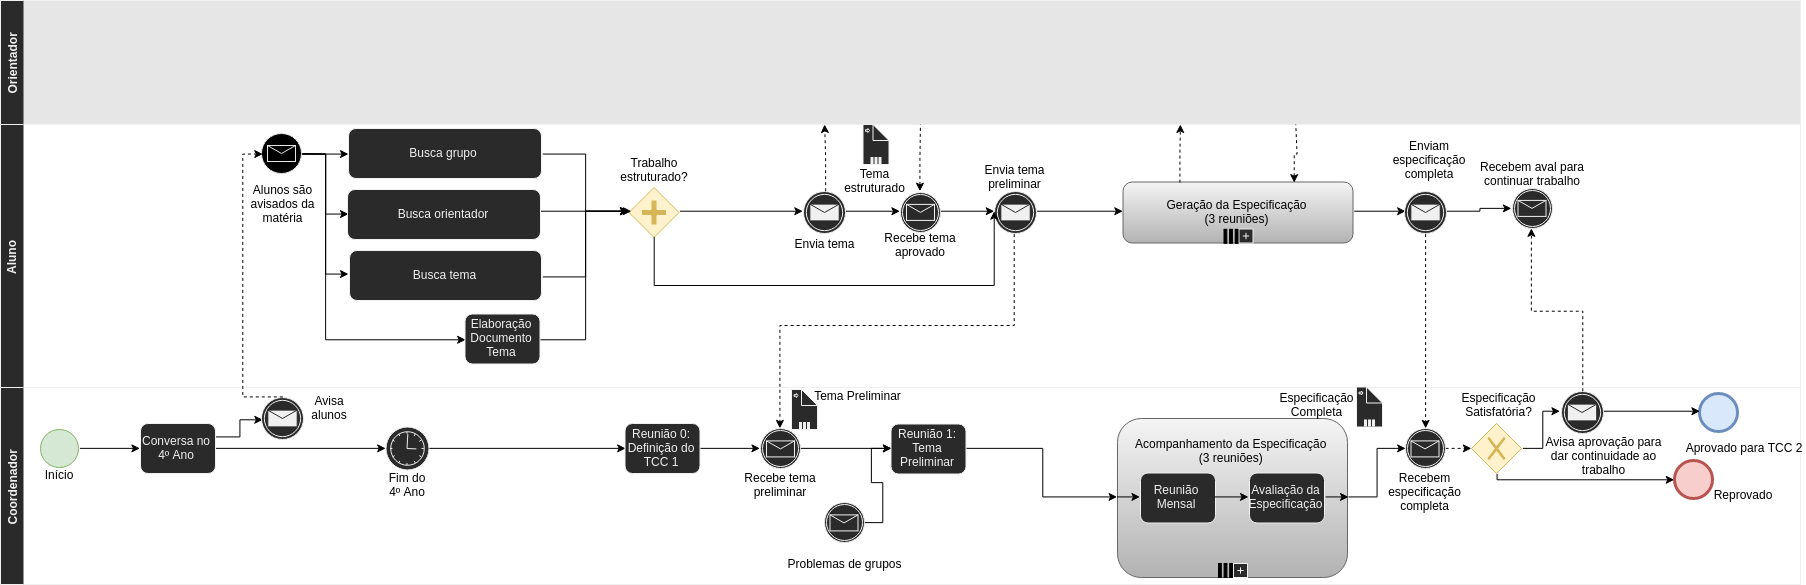
\includegraphics[angle=90, origin=c, scale=0.35]{bpmn-tcc1.png}
    \caption{Diagrama BPMN para a disciplina de TCC 1}
    \label{fig:bpmn-tcc1}
\end{figure}

\subsection{TCC 2}
\begin{figure}[H]
    \centering
    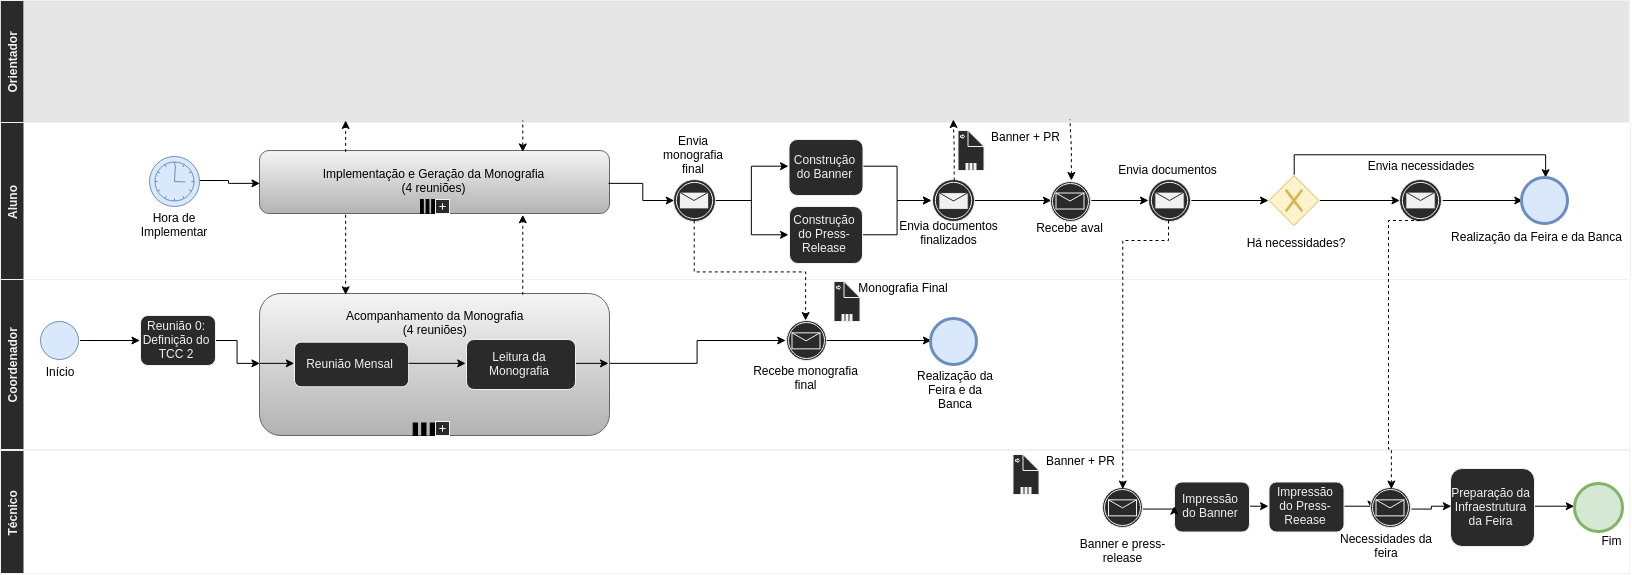
\includegraphics[angle=90, origin=c, scale=0.35]{bpmn-tcc2.png}
    \caption{Diagrama BPMN para a disciplina de TCC 2, antes dos eventos finais}
    \label{fig:bpmn-tcc2}
\end{figure}

\subsection{Banca e Feira}
\begin{figure}[H]
    \centering
    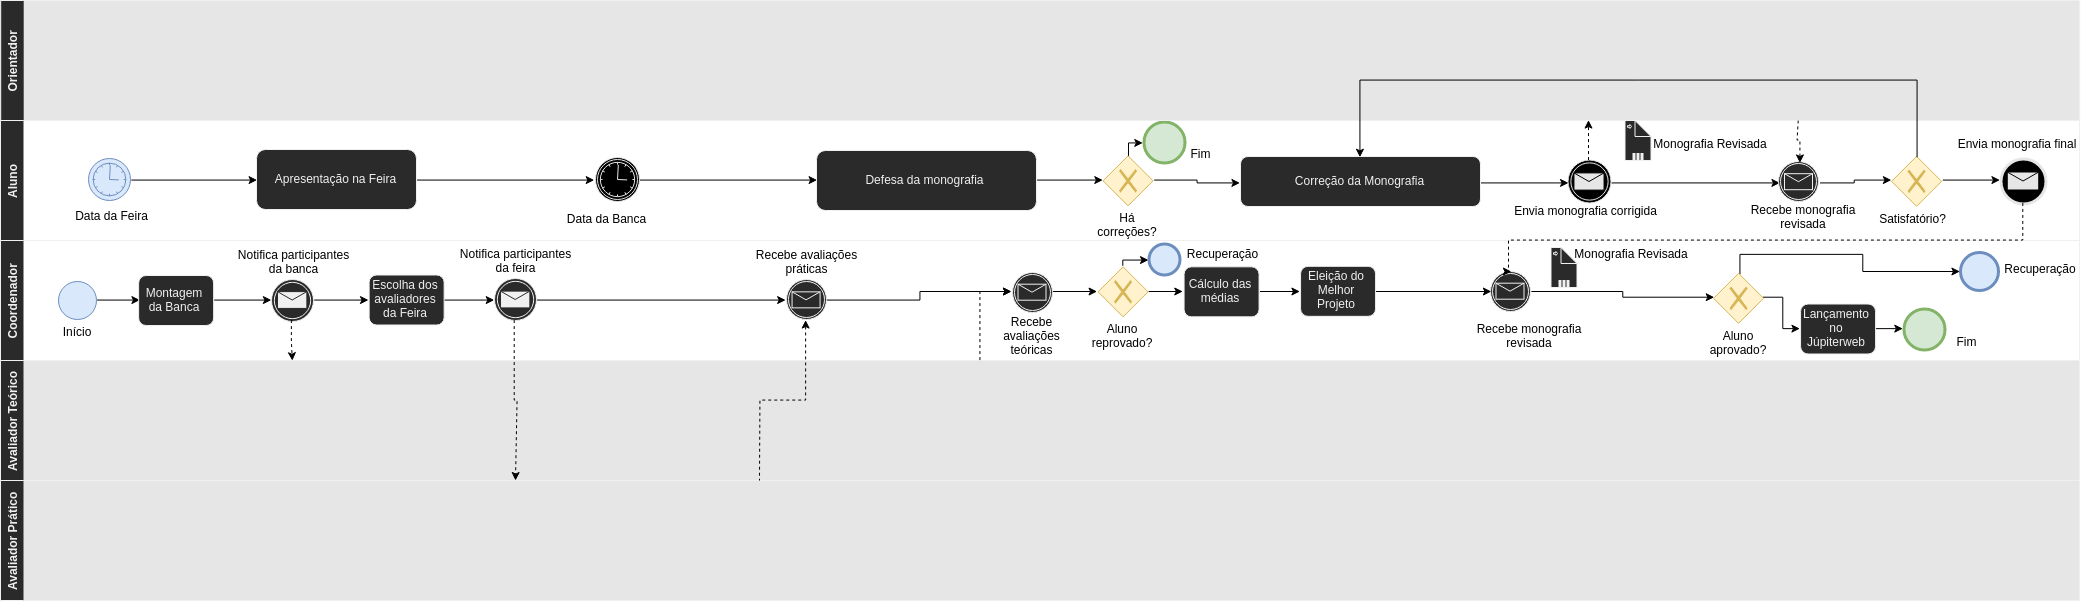
\includegraphics[angle=90, origin=c, scale=0.3]{bpmn-banca-feira.png}
    \caption{Diagrama BPMN para os eventos de banca e feira}
    \label{fig:bpmn-banca-feira}
\end{figure}

\subsection{Recuperação}
\begin{figure}[H]
    \centering
    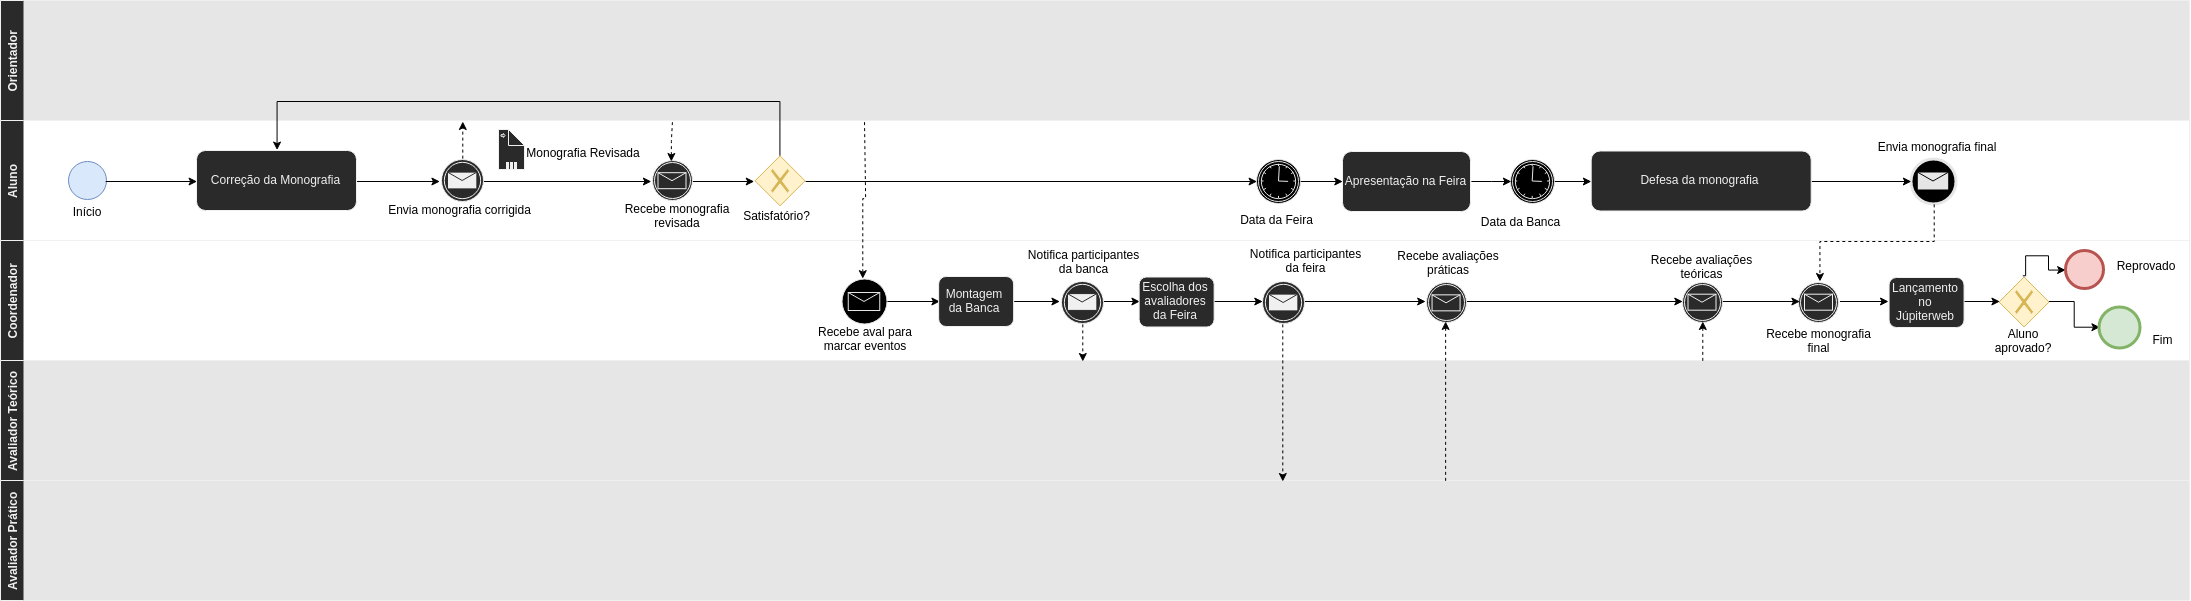
\includegraphics[angle=90, origin=c, scale=0.28]{bpmn-rec.png}
    \caption{Diagrama BPMN para a recuperação da disciplina de TCC 2}
    \label{fig:bpmn-rec}
\end{figure}

\chapter{Casos de Uso}\label{chap:use-case-appendix}
Neste apêndice consta os casos de uso escritos para o sistema em questão, usando o padrão explicado no capítulo de casos de uso\cite{ibm2011}. Para economizar espaços, campos ausentes nos casos de uso não foram explicitados.

\section{Cadastrar disciplinas}
\begin{enumerate}
    \item Breve Descrição: Coordenadores cadastram a disciplina, os alunos participantes e as atividades.
    \item Fluxo Básico:
        \begin{itemize}
            \item Coordenador insere disciplina, com os seguintes dados:
            \begin{itemize}
                \item Modalidade (Sem/Quad)
                \item Data de início e data de término
            \end{itemize}
            \item Coordenador importa planilha com alunos participantes, com os seguintes dados dos alunos
            \begin{itemize}
                \item Nome
                \item E-mail
                \item Nº USP
            \end{itemize}
            \item Coordenador insere uma nova atividade da disciplina, com os seguintes dados
            \begin{itemize}
                \item Nome
                \item Data de entrega e arquivos relacionados
                \item Peso da atividade
            \end{itemize}
            \item Sistema salva alunos novos, dispara e-mail ao aluno com seu acesso (login e senha) e vincula os existentes à disciplina e salva a disciplina
        \end{itemize}
    \item Fluxos Alternativos:
    \begin{enumerate}
        \item Data de início é posterior a de término
        \begin{enumerate}
            \item Sistema exibe novamente tela de cadastro da disciplina, alertando sobre erro
        \end{enumerate}
        \item E-mail é inválido
        \begin{enumerate}
            \item Sistema exibe novamente tela de cadastro da disciplina, alertando sobre erro
        \end{enumerate}
        \item E-mail retornou
        \begin{enumerate}
            \item Sistema envia e-mail ao coordenador com o aluno problemático
        \end{enumerate}
    \end{enumerate}
    \item Pré-condição: Coordenador deve estar logado
\end{enumerate}

\section{Editar disciplinas}
\begin{enumerate}
    \item Breve Descrição: Coordenadores editam disciplinas, cadastrando atividades, editando alunos etc.
    \item Fluxo Básico:
        \begin{itemize}
            \item Coordenador edita início e término da disciplina, alunos participantes, com novos alunos ou removendo os já participantes
            \item Coordenador insere uma nova atividade da disciplina, com os seguintes dados
            \begin{itemize}
                \item Nome
                \item Data de entrega
                \item Arquivos relacionados
                \item Peso da atividade
            \end{itemize}
            \item Sistema salva novas atividades e as mudanças da disciplina
        \end{itemize}
    \item Pré-condição: Coordenador deve estar logado
\end{enumerate}

\section{Cadastrar professores}
\begin{enumerate}
    \item Breve Descrição: Coordenadores cadastram professores do departamento que podem orientar/co-orientar.
    \item Fluxo Básico:
    \begin{itemize}
        \item Coordenador insere os dados do professor
        \begin{itemize}
            \item Nome
            \item Número USP
            \item E-mail
        \end{itemize}
        \item Sistema salva o professor, disparando e-mail para o professor cadastrado
    \end{itemize}
    \item Pré-condição: Coordenador deve estar logado
\end{enumerate}

\section{Cadastrar convidados externos}
\begin{enumerate}
    \item Breve Descrição: Coordenadores cadastram convidados externos do departamento que podem co-orientar.
    \item Fluxo Básico:
    \begin{itemize}
        \item Coordenador insere os dados do convidado externo
        \begin{itemize}
            \item Nome
            \item Empresa
            \item E-mail
        \end{itemize}
        \item Sistema salva o convidado externo, disparando e-mail para o convidado cadastrado
    \end{itemize}
    \item Pré-condição: Coordenador deve estar logado
\end{enumerate}

\section{Cadastrar grupos de trabalhos}
\begin{enumerate}
    \item Breve Descrição: Coordenadores cadastram os grupos com os temas e os orientadores, com a confirmação da participação do orientador no grupo.
    \item Fluxo Básico:
    \begin{itemize}
        \item Coordenador insere os dados do grupo
        \begin{itemize}
            \item Título
            \item Alunos
            \item Orientador
            \item Co-orientador
        \end{itemize}
        \item Sistema salva grupo e envia e-mail para o orientador, co-orientador e alunos
        \item Orientador valida participação no grupo
        \item Co-orientador valida participação no grupo
    \end{itemize}
    \item Fluxos Alternativos:
    \begin{enumerate}
        \item Grupo não tem orientador
        \begin{enumerate}
            \item Sistema cadastra grupo, enviando e-mail para os alunos com o aviso de urgência na escolha do orientador
        \end{enumerate}
        \item Grupo não tem aluno
        \begin{enumerate}
            \item Sistema retorna para a tela de cadastro de grupo, avisando sobre o erro de ausência de alunos
        \end{enumerate}
    \end{enumerate}
    \item Pré-condição: Coordenador deve estar logado, alunos, orientadores e co-orientadores cadastrados
    \item Pós-condição: Grupo confirmado
\end{enumerate}

\section{Login}
\begin{enumerate}
    \item Breve Descrição: Alunos, Orientadores, Co-orientadores e Coordenadores acessam sistema de maneira tradicional ou via Senha Única USP (para pertencentes à USP).
    \item Fluxo Básico:
    \begin{itemize}
        \item Sistema mostra campos de login e senha
        \item Usuário insere seu e-mail e sua senha
        \item Sistema valida e-mail e senha
        \item Usuário acessa sistema
    \end{itemize}
    \item Fluxos Alternativos:
    \begin{enumerate}
        \item Usuário erra credenciais
        \begin{enumerate}
            \item Sistema retorna para tela de acesso ao sistema, exibindo mensagem de erro
            \item Retorna normalmente à situação de mostrar campos de login e senha
        \end{enumerate}
        \item Usuário realiza login pela Senha Única da USP
        \begin{enumerate}
            \item Usuário seleciona $``$Acessar pela Senha Única USP$"$ 
            \item Usuário é redirecionado para os sistemas USP
            \item Retorna para a situação de acesso ao sistema
        \end{enumerate}
    \end{enumerate}
    \item Requisitos Especiais: Integração via Shibboleth com os Sistemas USP
    \item Pós-condição: Usuário dentro do sistema
\end{enumerate}

\section{Entregar atividade}
\begin{enumerate}
    \item Breve Descrição: Alunos submetem no Google Drive arquivos da atividade para a leitura do orientador, co-orientador e coordenadores. Orientador e co-orientador revisam e dão seu aval de aprovação com a documentação.
    \item Fluxo Básico:
    \begin{itemize}
        \item Aluno submete arquivos nos respectivos espaços de atividades, que são carregados no Google Drive e deixa comentários adicionais sobre a entrega
        \item Sistema salva a entrega com o status da entrega da atividade para $``$Não avaliada$"$
        \item Sistema envia e-mail para Orientador e Co-orientador avisando de submissão
        \item Orientador baixa documentos submetidos
        \item Orientador avalia a entrega, faz comentários aos alunos e comentários exclusivos à coordenação com notas
        \item Sistema salva entrega e dispara e-mail com o resultado da avaliação para os alunos
    \end{itemize}
    \item Fluxos Alternativos:
    \begin{enumerate}
        \item Data de submissão expirou (1)
        \begin{enumerate}
            \item Aluno não consegue interagir com atividade, encerrando fluxo
        \end{enumerate}
        \item Co-orientador realiza fluxo de revisão, antes do Orientador (4)
        \begin{enumerate}
            \item Passos 5 - 7 ocorrem normalmente, trocando Orientador por Co-orientador
        \end{enumerate}
        \item Co-orientador realiza fluxo de revisão, após Orientador (8)
        \begin{enumerate}
            \item Sistema exibe detalhes da entrega, porém não permite edições do lado do Co-orientador, encerrando fluxo
        \end{enumerate}
        \item Aluno submete nova entrega da atividade após ter feito uma submissão (1)
        \begin{enumerate}
            \item Aluno vê status da avaliação
            \item Aluno realiza nova entrega da atividade, repetindo o caso de uso
        \end{enumerate}
        \item Aluno submete entrega da atividade quando alguém do grupo já submeteu (1)
        \begin{enumerate}
            \item Sistema exibe detalhes da entrega já realizada
            \item Aluno pode realizar nova entrega da atividade, passando por cima da entrega anterior e repetindo o caso de uso
        \end{enumerate}
    \end{enumerate}
    \item Pré-condição: Atores devem estar autenticados e atividade deve estar cadastrada no sistema
\end{enumerate}


\section{Construir bancas práticas}
\begin{enumerate}
    \item Breve Descrição: Coordenadores selecionam os participantes da banca prática, já cadastrados no sistema, e os notifica com comentários sobre o evento.
    \item Fluxo Básico:
    \begin{itemize}
        \item Coordenador informa o dia da feira, a disciplina correspondente e as salas disponíveis para o evento, além de determinar o peso da avaliação da banca
        \item Sistema salva evento
        \item Coordenador seleciona evento recém criado.
        \item Sistema lista grupos do evento.
        \item Coordenador seleciona o grupo que deseja atribuir a sala e os convidados.
        \item Coordenador seleciona os convidados que avaliarão o grupo
        \item Sistema salva banca e envia e-mail para os convidados externos, avisando-os sobre sua participação
        \item Convidado acessa sistema e confirma participação na banca
    \end{itemize}
    \item Pré-condição: Atores devem estar autenticados e grupo de trabalho deve estar cadastrado no sistema
\end{enumerate}

\section{Construir bancas teóricas}
\begin{enumerate}
    \item Breve Descrição: Coordenadores escolhem participantes da banca teórica do grupo, selecionam o presidente da banca, realizam o agendamento do horário, validando inconsistências (participante já possui horário ocupado) e notificam os participantes por e-mail.
    \item Fluxo Básico:
    \begin{itemize}
        \item Coordenador informa o dia da banca, a disciplina correspondente e as salas disponíveis para o evento
        \item Sistema salva evento
        \item Coordenador seleciona evento recém criado.
        \item Sistema lista grupos do evento.
        \item Coordenador seleciona o grupo que deseja atribuir a sala e os convidados.
        \item Coordenador seleciona os avaliadores da banca e o horário da avaliação. O orientador é um dos pré-selecionados por padrão
    \end{itemize}
    \item Fluxos Alternativos:
    \begin{enumerate}
        \item Convidado externo já possui banca nesse dia e horário
        \begin{enumerate}
            \item Sistema barra criação de banca, alertando sobre qual convidado já possui agenda ocupada
        \end{enumerate}
        \item Sala está ocupada no horário selecionado
        \begin{enumerate}
            \item Sistema barra criação de banca, alertando sobre qual sala já possui agenda ocupada
        \end{enumerate}
    \end{enumerate}
    \item Pré-condição: Atores devem estar autenticados e grupo de trabalho deve estar cadastrado no sistema
\end{enumerate}

\section{Listar entregas}
\begin{enumerate}
    \item Breve Descrição: Técnicos recebem os arquivos de impressão, com normalização do título, separados por grupo.
    \item Fluxo Básico:
    \begin{itemize}
        \item Coordenador lista todas as entregas finais de impressão (\textit{banner} e \textit{press-release})
        \item Sistema salva as listas de arquivos finais, com o nome normalizado e envia por e-mail para o técnico responsável
    \end{itemize}
    \item Fluxos Alternativos:
    \begin{enumerate}
        \item Grupo de trabalho está com arquivo faltante
        \begin{enumerate}
            \item Sistema envia e-mail para o grupo com entrega faltante, avisando para regularizar a situação com urgência.
        \end{enumerate}
    \end{enumerate}
    \item Pré-condição: Atores devem estar autenticados e grupo de trabalho deve estar cadastrado no sistema
\end{enumerate}

\section{Listar necessidades adicionais}
\begin{enumerate}
    \item Breve Descrição: Técnicos recebem necessidades adicionais revisadas pelos orientadores, separadas por grupo.
    \item Fluxo Básico:
    \begin{itemize}
        \item Coordenador lista todos os comentários das entregas finais
        \item Sistema salva a lista de comentários e a envia por e-mail para o técnico responsável
    \end{itemize}
    \item Pré-condição: Atores devem estar autenticados e grupo de trabalho deve estar cadastrado no sistema
\end{enumerate}

\section{Avaliar projetos práticos}
\begin{enumerate}
    \item Breve Descrição: Participantes da banca prática avaliam os projetos que estão envolvidos, limitando avaliações até o final do dia.
    \item Fluxo Básico:
    \begin{itemize}
        \item Convidado externo acessa espaço da banca, com detalhes do grupo e as entregas finais
        \item Convidado preenche os comentários e as notas de acordo com cada critério estabelecido para avaliação de bancas práticas
        \item Convidado salva avaliação
    \end{itemize}
    \item Fluxos Alternativos:
    \begin{enumerate}
        \item Convidado tenta submeter avaliação em dia diferente ao da banca prática
        \begin{enumerate}
            \item Avaliação é barrada, avisando o convidado de que a avaliação só pode ser feita exclusivamente no dia
        \end{enumerate}
    \end{enumerate}
    \item Pré-condição: Atores devem estar autenticados e grupo de trabalho deve estar cadastrado no sistema
\end{enumerate}


\section{Avaliar monografias teóricas}
\begin{enumerate}
    \item Breve Descrição: Participantes da banca teórica avaliam as monografias que estão envolvidas, gerando comentários e definindo o status do trabalho (aprovado, aprovado com correções, recuperação e reprovado), limitando avaliações até o final do dia.
    \item Fluxo Básico:
    \begin{itemize}
        \item Participante da banca acessa espaço da banca, com detalhes do grupo e as entregas parciais e finais.
        \item Participante preenche os comentários e as notas de acordo com cada critério estabelecido para avaliação de bancas teóricas.
        \item Participante salva avaliação, com seu parecer para aprovação da monografia.
        \item Sistema usa a média das avaliações da banca para determinar o estado do grupo.
    \end{itemize}
    \item Pré-condição: Atores devem estar autenticados e grupo de trabalho deve estar cadastrado no sistema
\end{enumerate}


\section{Calcular nota final dos projetos}
\begin{enumerate}
    \item Breve Descrição: Coordenadores determinam a fórmula para calcular as notas finais, com base nas entregas parciais durante as duas disciplinas e o sistema calcula as notas finais de todos os grupos participantes.
    \item Fluxo Básico:
    \begin{itemize}
        \item Coordenador escolhe a disciplina de TCC2, a banca teórica e a feira prática que deseja obter as entregas
        \item Sistema salva fórmula de avaliação
        \item Sistema lista todos os grupos, com as notas calculadas e os estados de avaliação de cada grupo
    \end{itemize}
    \item Fluxos Alternativos:
    \begin{enumerate}
        \item Coordenador não preenche algum dos campos necessários
        \begin{enumerate}
            \item Sistema barra criação de fórmula de avaliação, avisando os campos faltantes
        \end{enumerate}
        \item Grupo tem alguma avaliação faltante
        \begin{enumerate}
            \item Sistema exibe grupo, mas com campo de Não Avaliado
        \end{enumerate}
        \item Grupo vai para recuperação na avaliação da banca teórica
        \begin{enumerate}
            \item A nota calculada é a nota da banca teórica, passando todas as outras avaliações realizadas ao longo das disciplinas
        \end{enumerate}
        \item Grupo é reprovado na avaliação da banca teórica
        \begin{enumerate}
            \item A nota calculada é a nota da banca teórica, passando todas as outras avaliações realizadas ao longo das disciplinas
        \end{enumerate}
    \end{enumerate}
    \item Pré-condição: Atores devem estar autenticados e grupo de trabalho deve estar cadastrado no sistema
\end{enumerate}


% ========== Anexos (opcional) ==========
\anexo

\end{document}
